\documentclass[main.tex]{subfiles}

\pagestyle{fancy}
\fancyhf{}
\fancyhead[LE]{\makebox[\pageoffset][l]{\bfseries\thepage}\bfseries\leftmark}
\fancyhead[RO]{\bfseries\rightmark\makebox[\pageoffset][r]{\bfseries\thepage}}

\begin{document}

\section*{Goal}
Today we will investigate the angular counterpart to force, torque. In our experiments we will see how the placement of the applied force can affect the torque on an object and how torque on an object affects the rotational dynamics on that object.

\section*{Equipment}
\begin{itemize}
\item
PASCO Capstone Software
\item
850 Universal Interface (850UI)
\item
Pegboard levers
\item
Masses
\item
Meter stick
\item
String
\item
Support frame
\item
Torque problem at lecture table
\item
Rotary Motion Sensor (RMS) and small pulley to be mounted on RMS
\item
Silver Disk, White Disk
\item
Triple-beam Balance
\end{itemize}•

\section*{Theory}

\begin{wrapfigure}{r}{0.5\textwidth}
\centering
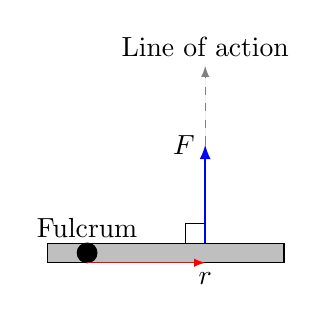
\begin{tikzpicture}[
	force/.style={thick,>=latex,draw=blue,fill=blue},
	axis/.style={dashed,>=latex,draw=gray,fill=gray},
	radial/.style={>=latex,draw=red,fill=red}
]
%\draw[help lines] (0,0) grid (3,3);
	\draw[fill=lightgray] (0,0) rectangle (3,0.25);
	\draw[fill=black] (0.5,0.125) circle [radius=0.125] node [above,yshift=2pt] {Fulcrum};
	
	\draw[force,->] (2,0.25) -- (2,1.5) node [left] {$F$};
	\draw[axis,->] (2,1.5) -- (2,2.5) node [above] {Line of action};
	\draw[radial,->] (0.5,0) -- (2,0) node [below] {$r$};
	
	\draw (1.75,0.25) -- (1.75,0.5) -- (2,0.5);
\end{tikzpicture}
\caption{} \label{fig:Torque}
\end{wrapfigure} \vspace{-10pt}

When we apply a force on an elongated object a distance $r$ from some point of rotation we will create a torque on the object. As in Figure~\ref{fig:Torque} the point that the body rotates around is called the fulcrum. The force $F$ on the object is applied along a line we call the ``Line of action." The distance $r$ is called the lever arm which is always measured \emph{from} the fulcrum \emph{to} the line of action of the force. In general the torque vector of the force with respect to the fulcrum is defined as,
\begin{equation} \label{eq:VectTorque}
\boldsymbol{\tau}=\mathbf{r} \times \mathbf{F},
\end{equation}
where this is the vector product of the vectors $\mathbf{r}$ and $\mathbf{F}.$ One of the properties of vector products is that the resultant must always be \emph{orthogonal} or mutually perpendicular to both parent vectors, so we can handle the direction and magnitude of our torque separately. The magnitude of torque is,
\begin{equation} \label{eq:MagTorque}
\tau=rF\sin\theta,
\end{equation}
where $\theta$ is the angle between the vectors $\mathbf{r}$ and $\mathbf{F}.$ For most of our experiment $\theta=\pi/2$ so Equation~\eqref{eq:MagTorque} simplifies to,
\begin{equation} 
\tau=rF.
\end{equation}

To determine the direction of the torque we use what is known as the ``right-hand rule." This simple mnemonic is true for all vector products and is setup as follows: The index finger of the right hand is pointed in the direction of the first vector of the product ($\mathbf{r}$), the middle finger is pointed in the direction of the second vector ($\mathbf{F}$), then the thumb will be pointing in the correct direction of the resultant vector ($\boldsymbol{\tau}$).
% Try to find an image of the Right-Hand Rule

It is worth to note that for a body that is in translational and rotational equilibrium, meaning that the the sums of the forces and the torques are both zero, the point that we choose for the fulcrum is arbitrary. We can choose any point on the body and the sum of the torques will still be zero. This is extremely advantageous for us because we can then choose a fulcrum that makes our calculations easier.

To study dynamic toque we first need to expand on what we stared in Chapter~\ref{chap:Cen_Force}. We had from equation~\eqref{eq:Vomega},
\begin{equation}\label{eq:Vomega_Torque}
v=\omega r.
\end{equation}
We also know that acceleration is the change in velocity, thus we can write our tangential acceleration in terms of angular acceleration $\alpha,$
\begin{equation}\label{eq:Aalpha}
a_{tan}=\frac{dv}{dt}=\frac{d}{dt}(r\omega)=r\frac{d\omega}{dt}=r\alpha.
\end{equation}
Now we can return to equation~\eqref{eq:MagTorque} and identifying that $F\sin\theta$ picks out the component of the applied force tangential to the angular motion we have,
\begin{equation}\label{eq:PartTorque}
\tau=rF_{tan}=r(ma_{tan})=rm(r\alpha)=mr^2\alpha.
\end{equation}
Since our body is a rigid object we can consider it as a collection of small pieces. Each piece of mass $m_i$ will rotate around a circle centered on the axis of rotation with the torque on each particle given by equation~\eqref{eq:PartTorque}. Thus the net torque on the entire body will be the sum of the individual torques,
\begin{equation} \label{eq:TorqueIalpha}
\sum \tau=\left(\sum m_ir_i^2\right)\alpha=I\alpha,
\end{equation}
where we define $I=\sum m_ir_i^2$ to be the moment of inertia of the body and describes how mass is distributed around a rotating body. We will explore the concept of moments of inertia in more detail in Chapter~\ref{chap:AngMom}.

\section{Setup I: Static Torque}
\subsection*{Procedure}
\begin{enumerate}
\item
Support the pegboard lever at the center by hanging it on a string attached to a hook ring. Verify that the board is approximately balanced in horizontal position at that point.
\item
Attach a 200 g mass to the third hole from the center using the lower line of holes. Calculate the mass needed at the sixth hole from the center on the opposite side to again balance the board. Hang that mass from the board and test for balance. Remember that there are uncertainties involved and make a list of their causes.
\item
Remove the last mass added and calculate what mass must be added at the fourth hole from the center on the side opposite the 200 g mass to re-balance the board. After testing the result, derive a simple formula that works for any situation.
\item \label{step:LeverBoard_start}
Remove all added masses and move the supporting string to the sixth hole from the center on the top row of holes. Add enough mass at the eighth hole on the same side to balance the lever board. Recall that the weight of the board can be approximated to a point at the center, use the formula derived in the previous step to determine  the mass of the board.
\item \label{step:LeverBoard_end}
Use the triple-beam balance to measure the mass of the lever board.
\item
At the lecture desk is a rod and ball setup that is in rotational equilibrium. Record the scale values (in the proper units) and angles of the supporting strings using the protractor available. Make all length measurements deemed necessary to determine the mass of the bar and the mass of the ball hanging from the bar. Assume the center of the mass of the bar is at the center of the bar.
\end{enumerate}•

\subsection*{Analysis}
\begin{enumerate}
\item
Determine the relative discrepancy in the mass of the lever board by comparing the results from steps~\ref{step:LeverBoard_start}--\ref{step:LeverBoard_end}.
\item
Determine the mass of the bar and the ball hanging from the bar.
\end{enumerate}•

\begin{question}
Explain why door handles are typically placed furthest from the hinges.
\end{question}

\begin{question}
Work is defined by the product of force and displacement while torque is defined by the product of force and distance. Are work and torque equivalent? Explain why or why not.
\end{question}

\section{Setup II: Dynamic Torque}
For this setup, we will use the Rotary Motion Sensor (RMS) to measure the angular acceleration of our system which when combined with other measurements will allow us to determine the torque on the system.
\begin{enumerate}
\item
Open Capstone.
\item
Connect the RMS to the 850UI then setup Capstone to record from the sensor (click on the left-most port that the sensor is plugged into).
\item
Create a graph of Angular Acceleration vs Time.
\item
Mount the RMS on the vertical rod in the table so that the disks will be on top.
\item 
Tie the string around the smallest, top step of the clear plastic RMS pulley. Then, feed the string down through the notch into the middle step and wrap the string around the middle step.
\end{enumerate}•

\subsection*{Procedure}
\begin{enumerate}
\item
Measure the mass of the silver disk and record it. Measure the diameter of the silver disk three different times from different locations on the disk and record the average.
\item \label{step:Dyn_Torque_Start}
Attach the silver disk to the RMS.
\item
Lay the string over the black pulley at the end of the RMS.
\item
Attach the 50 g mass hanger (feel free to experiment with extra masses but 50 g should do the job) to the string.
\item
Click the Record button to start data collection and release the hanging mass.
\item
Stop data collection when the hanging mass is at its lowest point.
\item
Use the Selection Tool 
\includegraphics{Selection_Tool} to highlight the constant portion of the data corresponding to the string being unwound.
\item \label{step:Dyn_Torque_End1}
Display the mean and standard deviation of the data using the Statistics button 
\includegraphics{Statistics}. Record this into the data sheet.
\item 
Reset the RMS but this time wind the string around the lowest, largest step of the clear RMS pulley. The silver disk may need to be removed to access the pulley.
\item \label{step:Dyn_Torque_End2}
Repeat steps~\ref{step:Dyn_Torque_Start}--\ref{step:Dyn_Torque_End1} with the string on the larger step of the RMS pulley.
\item
We now want to see how changing the moment of inertia affects the measured torque. To do this we will replace the silver disk for the white disk. Measure the mass of the white disk an record it. Measure the diameter three times from different locations on the disk and record the average.
\item
Remove the silver disk, remember to return the screw to the RMS then place the white disk on the RMS.
\item
Repeat steps~\ref{step:Dyn_Torque_Start}--\ref{step:Dyn_Torque_End2}.
\item
Use the Select Data Run button 
\includegraphics{Select_Data_Run} to display all four runs. \textbf{Print} a copy of this graph for each group member.
\end{enumerate}•

\subsection*{Analysis}
\begin{enumerate}
\item
Calculate the moments of inertia for both the silver and white disks. The moment of inertia of a solid disk is given by,
\[
I_{disk}=\frac{1}{2}mr^2,
\]
where $r$ is the radius of the disk.
\item
Calculate the torque for each of the four runs above using equation~\eqref{eq:TorqueIalpha}.
\item
Average the torques for both disks that had the string around the smaller step of the RMS pulley. Repeat this for the torques at the larger step of the RMS pulley.
\end{enumerate}•

\begin{question}
How constant is the torque for runs on the same step of the RMS pulley? What is the relative discrepancy?
\end{question}

\begin{question}
Say we were to use a RMS pulley with an even larger radius than the large step on our pulley. How should the torque compare to our previous runs?
\end{question}

\begin{samepage}
\hrulefill \\
\emph{Chapter~\ref{chap:Torque}:} \textbf{Torque}
\begin{enumerate}
\item
\textbf{(1)} Title Page
\item
\textbf{(5)} Purpose
\item
\textbf{(10)} Theory---Should cover both setups
\item
\textbf{(5)} Procedure for Setup II
\item
\textbf{(2)} Graph
\item
\textbf{(4)} Data Sheet
\item
\textbf{(10)} Data Analysis with sample calculations shown.
\item
\textbf{(8)} Answers to all questions
\item
\textbf{(5)} Conclusion
\end{enumerate}•
\end{samepage}




\newpage
\begin{doublespace}
\section{Data Sheets}
\subsection*{Static Torque}
Mass needed to counter 200 g at third hole:\rule[-1mm]{2.5cm}{.1pt}\\
Uncertainties: \\[3cm]
Mass needed to counter 200 g at fourth hole:\rule[-1mm]{2.5cm}{.1pt}\\
Formula:\\[3cm]
Mass needed to counter weight of the board:\rule[-1mm]{2.5cm}{.1pt}\\
Mass of board (calculated):\rule[-1mm]{2.5cm}{.1pt}\\
Mass of board (measured):\rule[-1mm]{2.5cm}{.1pt}\\[1cm]
Lecture Desk Problem:\\
Force on string:\rule[-1mm]{2.5cm}{.1pt}, Angle:\rule[-1mm]{2.5cm}{.1pt}\\
Force on string:\rule[-1mm]{2.5cm}{.1pt}, Angle:\rule[-1mm]{2.5cm}{.1pt}\\
Sketch with lengths indicated:

\newpage
\subsection*{Dynamic Torque}
Mass of Silver Disk:\rule[-1mm]{2.5cm}{.1pt}\\
Average Diameter of Silver Disk:\rule[-1mm]{2.5cm}{.1pt}\\ \\
Mass of White Disk:\rule[-1mm]{2.5cm}{.1pt}\\
Average Diameter of White Disk:\rule[-1mm]{2.5cm}{.1pt}\\ \\


\begin{tabular}{c|c|c|}
\cline{2-3}
&\multicolumn{2}{|c|}{Angular Acceleration (rad/s$^2$)}\\
\hline
\multicolumn{1}{|c|}{Object} & Small Step & Large Step\\ \hline
\multicolumn{1}{|c|}{Silver Disk} &&\\ \hline
\multicolumn{1}{|c|}{White Disk}&&\\ \hline
\end{tabular}



\end{doublespace}

\end{document}
